% !TeX encoding=utf8
% !TeX spellcheck = de_CH_frami

\section*{Abstract}

%\todo{Abstract, Abstract Template: ZHAW\_FUP\_SEM\_IOT\_Abstract.tex}
\subsection*{Ausgangslage und Ziel}
Einer immer grösseren Beliebtheit erfreuen sich kleine Alltagsgegenstände welche mit dem Internet verbunden sind. Dieser Bereich wird \gls{acr:IOT} genannt. Diese Gegenstände / Geräte sind in der Lage Daten zu sammeln, speichern und weiterzuleiten. Da es zukünftig voraussichtlich immer mehr solcher \gls{acr:IOT} Geräte geben wird fallen immer mehr Daten an. Der Themenbereich des Aufbereiten, Aggregieren, Analysieren und Visualisierens dieser Daten wird auch als "`BigData"' bezeichnet.

Das Hauptziel dieser Arbeit ist die Überprüfung des Sachverhaltes, ob sich funktionale Programmiersprachen eigenen um Sensor-Daten auf einem \gls{acr:IOT} Gerät zu sammeln und anschliessend auszuwerten. Um diesen Sachverhalt zu prüfen, sollen mit einem \gls{acr:IOT} Gerät (Raspberry Pi) Sensor-Daten ermittelt und gespeichert werden. Anschliessend folgt eine Aufbereitung und Visualisierung der gespeicherten Daten.

\subsection*{Sensordaten sammeln}


\subsection*{Sensordaten aufbereiten und auswerten}

\subsection*{Resultat}

\begin{figure}[htb]
	\begin{subfigure}[b]{0.45\linewidth}
		\centering
		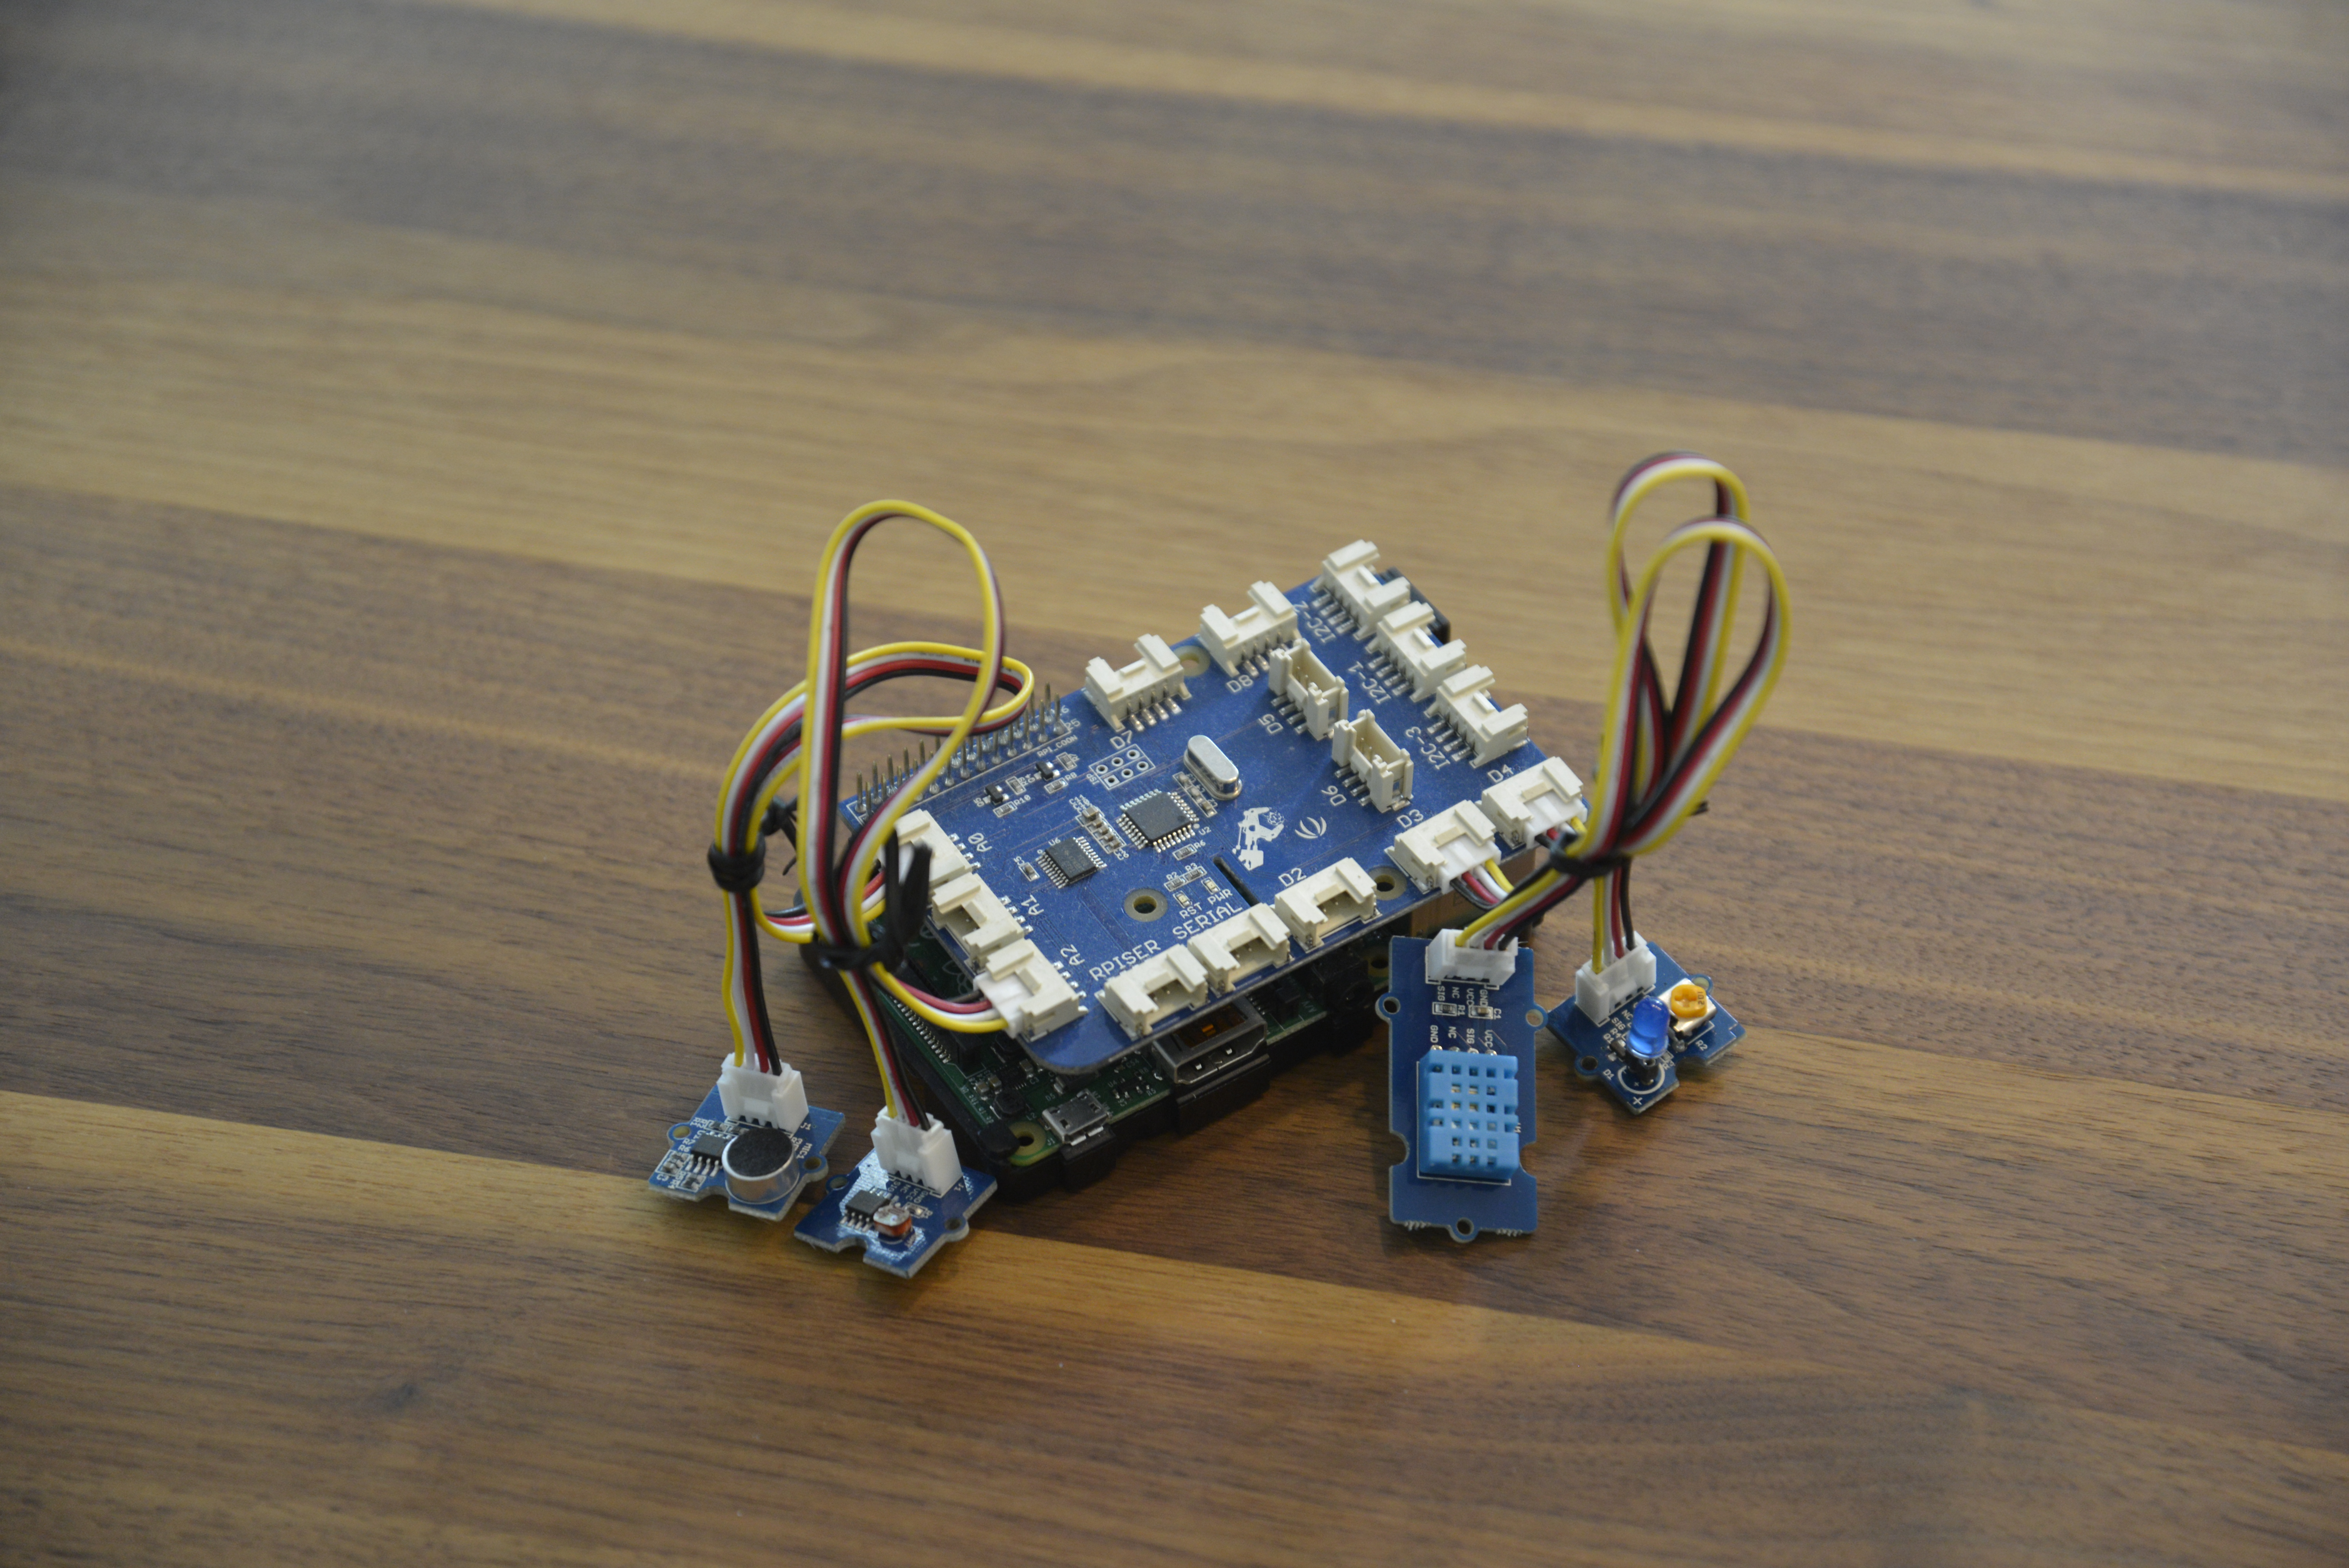
\includegraphics[width=6.5cm]{images/_DSC2012}
		\caption{Raspberry Pi mit GrovePi Board und Sensoren}
	\end{subfigure}
	\begin{subfigure}[b]{.45\linewidth}
		\centering
		\includegraphics[width=6.5cm]{images/resultat}
		\caption{Visualisierung der Daten}
	\end{subfigure}
\end{figure}
